\documentclass{report}
\usepackage{homework}
\usepackage{graphicx}
\usepackage[export]{adjustbox}
\solstrue

\definecolor{mygray}{gray}{0.95}
\usepackage{listings}
\lstset{
basicstyle=\small\ttfamily,
columns=flexible,
breaklines=true,
backgroundcolor = \color{mygray},
framexleftmargin = 1em,
xleftmargin = 1em
}

\renewcommand{\hmwkTitle}{Homework 5}

\begin{document}
\mktitle


\begin{problem}
\begin{figure}[!ht]
	\centering
	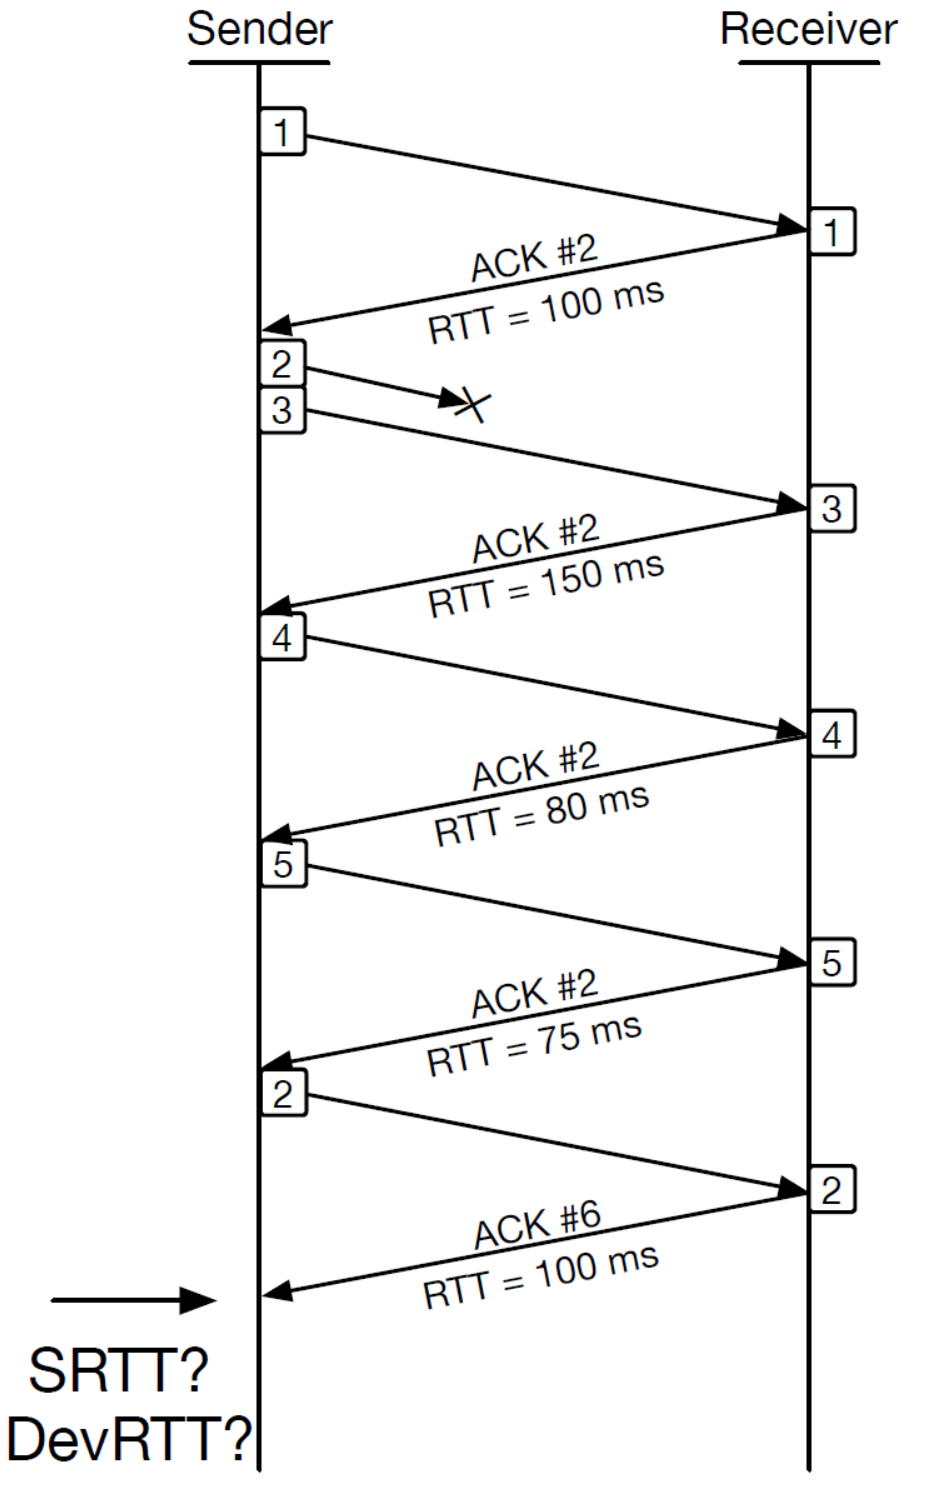
\includegraphics[valign=T,width=0.5\textwidth]{image1.png}
	\caption{TCP RTT estimation.}
	\centering
	\label{fig:image1}
\end{figure}

Calculate SRTT (RTT estimate), DevRTT, and RTO for a TCP connection shown in
Figure 1 \textbf{at the marked point of time}. Use standard initial default
parameters for the TCP connection (3 second for SRTT, 3 seconds for DevRTT),
and $\alpha = 1/8, \beta = 1/4$.\\
\indent Note that the second packet gets dropped during transmission and
retransmitted at a later time.

\begin{enumerate}
	\item SRTT = 100 ms
	\item DevRTT = 50 ms
	\item RTO = 300 ms
\end{enumerate}

\textbf{STUDENT NOTES:}
\begin{itemize}
  \item If we ignore that the ``ACK \#2''s might be ambiguous as to which
packet is being ACKed and assume we can still identify which packet this ACK
corresponds to (using, Selective ACKs), the values will be: SRTT = 99.472 ms,
DevRTT = 40.039 ms, and RTO = 259.629 ms.
  \item Assume that the ACK for packet 2 does not expire, per Piazza post.
  \item We retransmit packet 2 so we do not include the RTT for ACK \# 6
in our calculation.
\end{itemize}

\end{problem}

\clearpage
\begin{problem}

\begin{figure}[!ht]
	\centering
	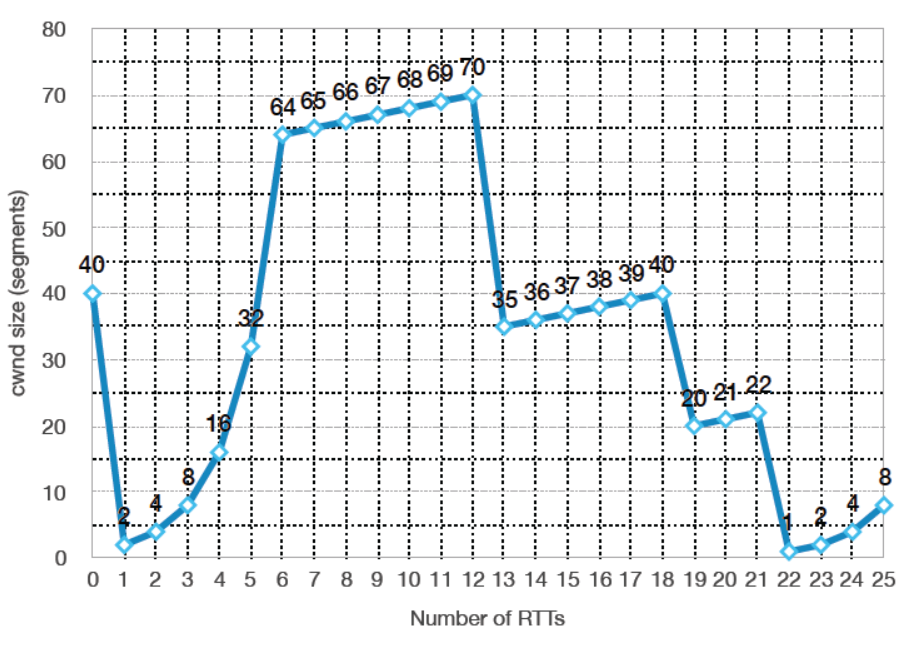
\includegraphics[width=0.5\textwidth]{image2.png}
	\caption{TCP congestion control.}
	\centering
	\label{fig:image2}
\end{figure}

Assume TCP Reno (with Fast Retransmit and Fast Recovery) is the protocol
experiencing the behavior shown above. Assume that the TCP flow has been
operating for some time, meaning that the number of RTTs shown are with respect
to when you started observing the flows behavior.

\begin{enumerate}
\item \textbf{On the graph above}, identify the time periods when TCP slow start
      is operating.
\item \textbf{On the graph above}, identify the time periods when TCP congestion
      avoidance is operating (AIMD).
\item For each loss event, specify whether it was detected by a triple duplicate
      ACK or by a timeout
\item For each loss event, indicate the value of the slow start threshold (ssthresh)
\end{enumerate}

\begin{answer}{25em}
  \begin{enumerate}
    \item TCP slow start is operating from RTTs 1--6 and RTTs 22--25.
    \item TCP congestion avoidance is operating from RTTs 6--12, 13--18, and
      19--21 (with TCP fast recovery inbetween these ranges).
    \item
      \begin{enumerate}
        \item Loss event 1, RTT 0: timeout (prof said to ignore this one)
        \item Loss event 2, RTT 12: triple ACK
        \item Loss event 3, RTT 18: triple ACK
        \item Loss event 4, RTT 21: timeout
      \end{enumerate}
    \item
      \begin{enumerate}
        \item Loss event 1: RTT 0: $ \texttt{ssthresh} = 20 $\\
              Don't know why slow start keeps increasing to 64 as the notes
              say that on timeout, \texttt{ssthresh} is set to 1/2
              \texttt{cwnd} = 1/2 (40) = 20.\\
              (prof said to ignore this one)
        \item Loss event 2: RTT 12: $ \texttt{ssthresh} = 35 $
        \item Loss event 3: RTT 18: $ \texttt{ssthresh} = 20 $
        \item Loss event 4: RTT 21: $ \texttt{ssthresh} = 11 $\\
              \texttt{ssthresh} = 1/2 \texttt{cwnd}
      \end{enumerate}
  \end{enumerate}
\end{answer}

\end{problem}

\clearpage
\begin{problem}

Consider transferring a large amount of data over the link with 10 Mbit/s
bandwidth using TCP Reno (only you're using the link at this time). Assuming
that losses in this link can only happen because of the buffer overflow, i.e.,
there are no random losses.
\begin{enumerate}
	\item Draw a diagram showing (approximately) how the sender’s cwnd changes
        over time.
	\item What is the maximum average throughput that this TCP flow can achieve?
\end{enumerate}

\begin{answer}{40em}
  \begin{enumerate}
    \item 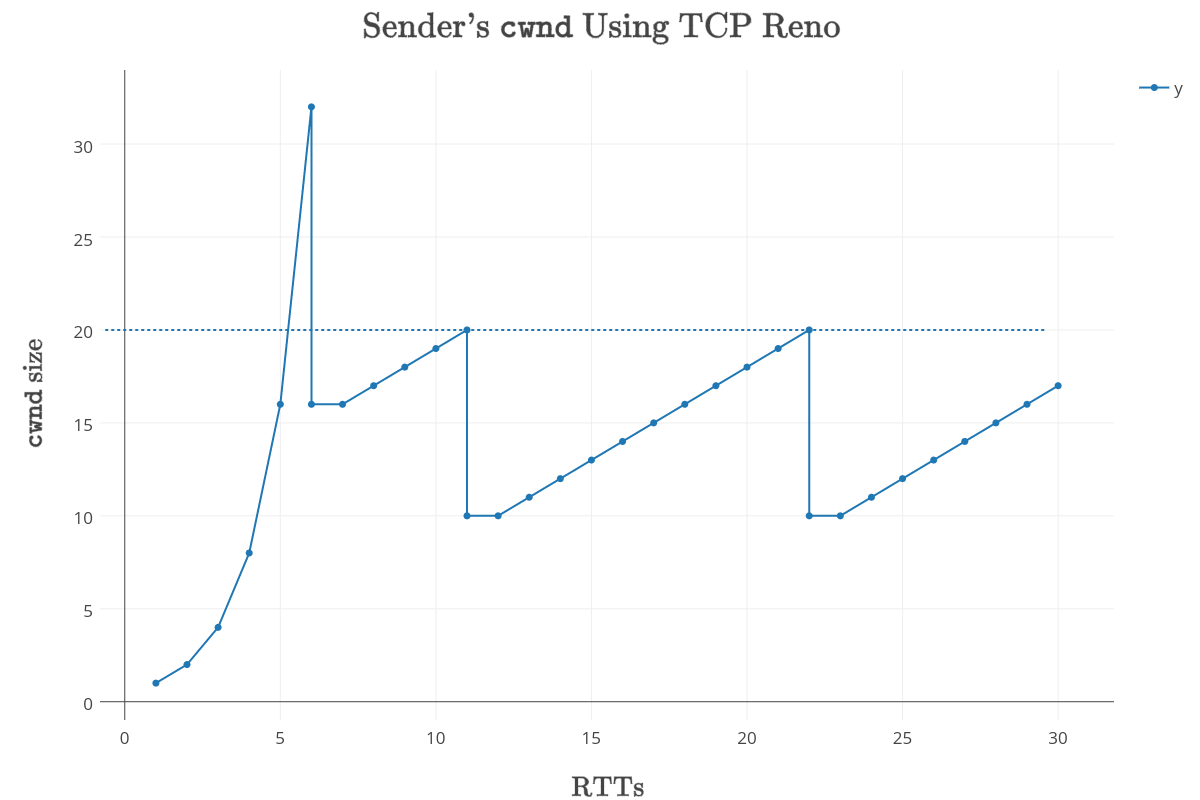
\includegraphics[valign=t,width=0.5\textwidth]{TCP-RENO}\\
          The blue dotted line represents the network bandwidth limit, such that
          a TCP connection fully utilizing the link would be consistently
          sending 20 MSS per RTT. We begin with slow start, which quickly
          surpasses the network limit, experiences multiple dropped packets,
          cuts \texttt{cwnd} by half and jumps into fast retransmit/fast
          recovery. 1 RTT later and we're in congestion avoidance, until we hit
          the network limit, lose a packet, cut \texttt{cwnd} in half again and
          repeat. This sawtooth pattern will repeat itself for the remainder of
          the connection, allowing us to make an estimate of the utilization of the link by TCP Reno.
    \item $\approx 3/4$ of the total available bandwidth (\textit{slightly}
           less). In the context of this problem, that would be 7.5 Mbit/s.
           Note that if there were multiple TCP connections on this link, on
           average this behavior would encourage full utilization of the link.
           Also note that in other cases the bandwidth can be calculated using:
             $$\text{bandwidth} = \frac{\text{window size}\cdot\text{MSS}}{\text{RTT}}$$
  \end{enumerate}
\end{answer}

\end{problem}


\clearpage
\begin{problem}

Suppose that two hosts are using TCP to communicate. They open a TCP connection
between them and start to send data. Assume that \texttt{ssthresh} is 64 KB and
the segment size is 3 KB.
\begin{enumerate}
	\item How many bytes are transmitted after 3 RTTs assuming no losses? Show
        your work.
	\item Now, suppose that after the third RTT, a loss occurs which results in
        the TCP sender timing out. What actions does TCP congestion control take?
	\item Assuming no losses will occur from then on, how many RTTs does it take
        to transmit an additional 22 KB of data?
\end{enumerate}

\begin{answer}{35em}
  TCP Tahoe and TCP Reno both take the same actions when an ACK times out, so
  this detail is not important to the problem.
  \begin{enumerate}
    \item 
      \begin{itemize}
        \item 1st RTT: \texttt{cwnd} = 1 MSS, 3KB are sent by the sender, 1 ACK received
        \item 2nd RTT: \texttt{cwnd} = 2 MSS, 6KB are sent by the sender, 2 ACKs received
        \item 3rd RTT: \texttt{cwnd} = 4 MSS, 12KB are sent by the sender, 4 ACKs received
        \item In the first 3 RTTs, a total of 21KB are exchanged.
      \end{itemize}

    \item 4th RTT: \texttt{cwnd} = 8 MSS, only 7 ACKs are received, the 8th ACK
          times out.\\
          TCP congestion control will respond by:
          \begin{itemize}
            \item \texttt{ssthresh} $\gets \frac{1}{2} \mathtt{cwnd} =$ 4 MSS
            \item \texttt{cwnd} $\gets$ 1 MSS
            \item Reinitiating slow start.
          \end{itemize}

    \item
      \begin{itemize}
        \item 5th RTT: \texttt{cwnd} = 1 MSS, 3KB are sent
        \item 6th RTT: \texttt{cwnd} = 2 MSS, 6KB are sent
        \item 7th RTT: \texttt{cwnd} = 4 MSS, 12KB are sent, enter Congestion Avoidance
        \item 8th RTT: \texttt{cwnd} = 5 MSS, 15KB are sent
      \end{itemize}
      In 4 more RTTs, we transmit 30 additional bytes of data (in 3 RTTs we
      transmitted only 21 bytes).
  \end{enumerate}
\end{answer}

\end{problem}


\end{document}
